\documentclass[a4paper]{article}
\usepackage{tikz}
\usepackage{mathtools}
\usepackage{caption}
\DeclarePairedDelimiter{\ceil}{\lceil}{\rceil}
\begin{document}
	\title{A Coexistence model of {IEEE} 802.11b/g {IEEE} 802.15.4 and {LTE-U}}
	\author{Harshavardhan Nalajala}
	\date{}
	\maketitle
	\tableofcontents
	
	\section{Problem Statement}
	Present a coexistence model of {IEEE} 802.11b/g, {IEEE} 802.15.4 and {LTE-U} to accurately explain their coexistence performances.
	
\section{Network Model}
	Consider a network consisting an {LTE-AP}, $N_{lte}$ {LTE} nodes, $N_{WiFi}$ 802.11b/g nodes, $N_{wsn}$ 802.15.4 nodes. Herein after 802.11b/g nodes are referred to as {WiFi} nodes and 802.15.4 nodes are referred to as {Wsn} nodes. {LTE} nodes and {LTE-AP} are expected to implement Fair LBT Algorithm described in \cite{7419263}. {LTE}, {WiFi} and {WSN} Iare saturated networks to simulate continuous contention for medium access. Physical channel is expected to be error free and the only packet drops are due to collisions. All nodes are in co-channel interference range. {WiFi} nodes are expected to sense {Wsn} and {LTE} powers of transmission while {Wsn} nodes can sense transmit power levels of {WiFi} and {LTE} nodes. All three networks' nodes use the same {2.4Ghz} channel and time share the medium to avoid interference and collisions. We now use this network model to understand and present a coexistence model of all three networks together.
	
\section{Motivation}
	Wireless communication has become core of mobile communications. {LTE} communications happen in licensed bands brought by mobile service providers. With increase in mobile users, service providers have started looking to provide {LTE} communications in unlicensed bands since these bands are not highly occupied compared to licensed bands. However, this introduced new challenges where {LTE} needs to co-operate with  incumbent technologies like {WiFi}, {Bluetooth} and {Wsn}. {LTE} when deployed without any modifications to its protocol in unlicensed band, would just kill the existing technologies in the same unlicensed band. To address such issues, {LTE} mac operation has been changed to on/off based duty cycling mode({LTE-U}). Many studies have been conducted on duty cycle based {LTE-U} and one of existing technologies in 2.4Ghz. {WiFi} and {Wsn} coexistence has been studied extensively and introduction of {LTE-U} as dominant technology in unlicensed band has triggered further studies. {LTE-U} and {WiFi} coexistence has been studied extensively while coexistence of {LTE-U} and {Wsn} has also been studied although not extensively. {WiFi} has become core part of every home, office. {Wsn} is being used for many sensor and battery critical operations. With {LTE} in licensed band, most cellular communications use LTE. With {LTE-U} in unlicensed band, there is a great need to study the coexistence behaviour of {LTE-U}, {WiFi} and {Wsn} in the same unlicensed band together since many networks have all three technologies operating together.
	
	\section{Introduction}
	Coexistence of various networks in unlicensed band has been the focus of study for a long time now. 802.11, 802.15.4 and Bluetooth coexistence has been studied extensively in \cite{953230}, \cite{4024941}, \cite{1666534}, \cite{7793984}, \cite{6425289}, \cite{4436237}, \cite{Tytgat2012}, \cite{6645003}. Other modes of interferences including microwave ovens, cordless phones have also been studied in \cite{5210929}. Recent advances have introduced {LTE} in unlicensed band and has led to extensive studies on coexistence of 802.11 or 802.15.4 with {LTE-U} and {LAA based LTE} in \cite{7564872}, \cite{7497766}, \cite{7419263}, \cite{7583669}, \cite{7063521}, \cite{7506714}.  802.11, 802.15.4 and {Bluetooth} are the most common networks deployed in {2.4Ghz}. \cite{7506714} discusses coexistence of {LTE} with {ZigBee} in {2.4Ghz}. Coexistence of these common networks together with {LTE-U} has not been studied thus far. {Bluetooth} has the option of jumping to non overlapping channel using {FHSS}. However {CSMA/CA} based 802.11 and 802.15.4 {MAC} layer operation needs to be studied together with {LTE-U} since {LTE-U} does not sense the channel before transmitting.\par
	Today, most protocols in unlicensed are implemented in the same mobile device with {WiFi} being used for internet primarily, {LTE} being used for mobile communications and {WSN} being used for transmitting sensor data. {WiFi} and {WSN} follow CSMA/CA based mac operations and can coexist among themselves in unlicensed band. {LTE}, being TDMA protocol in licensed band, does not interfere with {WiFi} and {WSN}. Now that {LTE} is being introduced in unlicensed band and since its a TDMA protocol with higher power of transmission that {WiFi}, interferes with {WiFi} and {WSN}. There is a need to study the behaviour of these protocols when they coexist and develop efficient coexistence models which maximise overall network performance and minimise overall collisions among protocols. Before we study the coexistence behaviour, let us understand the current protocol operations in the unlicensed bands.
\subsection{LTE operation in unlicensed band}
{LTE} operation in unlicensed band can be classified into two behaviours.
\begin{itemize}
\item Based on 3GPP Rel. 12, {LTE-U} is the unlicensed flavor of {LTE} protocol in licensed bands. {LTE} {TDMA} based mac operation is applied to {LTE-U} in unlicensed bands without any change in mac protocol behaviour. However, duty cycling is introduced so that other technologies get a share of the medium being used to transmit.
\item Licensed Assisted Access ({LAA}) is introduced in 3GPP release 13 as part of {LTE Advanced Pro}. It uses carrier aggregation in the downlink to combine {LTE} in unlicensed spectrum with LTE in the licensed band. It uses a contention protocol known as listen-before-talk (LBT), mandated in some European countries, to coexist with other Wi-Fi devices on the same band.
\end{itemize}

\subsection{WiFi operation in unlicensed band}
{WiFi} uses {CSMA/CA} based mac operation. It senses the channel for energy and transmit data if there is no energy in the medium for atleast few nano seconds({DIFS}). To avoid collisions, it uses binary expontial back-off ({BEB}) counter before transmitting. Back-off counter is frozen when the medium is busy and is resumed when the medium is idle. Once the back-off counter reaches zero, {WiFi} transmits.
\subsection{WSN operation in unlicensed band}
{WSN} uses {CSMA/CA} based operation similar to {WiFi} except that back-off counter is not frozen when the medium is busy. This protocol is mainly used for low powered devices.

\section{Classification of Coexistence Solutions}
Coexistence of networks in the same unlicensed band can be studied based on three modes of separation.
	\begin{itemize}
		\item Spatial separation where networks are separated out of co-channel interference range.
		\item Temporal separation where networks using the same frequency time share the medium to avoid interference and collisions.
		\item Frequency separation where networks use different channels avoiding interference.
	\end{itemize}
\subsection{Channel selection using spatial separation}
Devices separated from each other atleast out of co-channel interference range, can use the same channel for transmissions and reception of data. However, number of devices using wireless are growing day by day and spatial separation will not be a viable solution as number of devices grow.
\subsection{Channel selection using frequency separation}
Devices which are in the same co-channel interference range use different frequencies for transmission and reception of data. However, as density of devices grow in the same space, frequency separation will not be a viable solution due to the limited number of channels. Based on how channel selection happens, it can further be classified as
\begin{itemize}
\item Random channel selection where device selects a channel randomly and checks if any other device is using the same channel nearby.
\item Distributed channel selection where devices co-ordinate among themselves and select a channel based on the outcome of distributed co-ordination.
\item Centralized channel selection where a central authority, typically operator, assigns a channel to each device.
\end{itemize}
\subsection{Channel sharing using temporal separation}
Devices use the same channel in a time sharing fashion. Performance of the network is dependent on effective time sharing the channel. 
 Coexistence can further be classified based on the mac operations of the protocols sharing the same channel.
\begin{itemize}
\item Mac Operation based on duty cycling
A duty cycle is the fraction of one period in which a signal or system is active. A mac protocol using this mechanism has on and off periods. During on period, it transmits and receives data. During off period, it turns the transmission off and sleeps. Other protocols sharing the same channel can transmit/receive during its off period. {LTE-U} uses duty cycling based mechanism to coexist with other technologies in unlicensed band with the help of idle subframes in its frames.

\item Mac operation based on Listen Before Talk({LBT})
Listen Before Talk (LBT) or sometimes called Listen Before Transmit is a technique used whereby a radio transmitters first sense its radio environment before it starts a transmission.
{WiFi, WSN and Licensed Assisted Access (LAA) based LTE use this}. Mac protocol listens to channel for energy, determines if the channel is idle. If the channel is idle for a period of time, it transmits. If the channel is not idle, it does not transmit and waits for the channel to become idle.
\end{itemize}
As technology advances, number of mac operations a device supports are increasing there by increasing the density of devices in the same area. It is imperative that eventually devices end up sharing the channel with temporal separation.  Number of mobile communication devices using the channels has become so large that even after frequency separation we end up with time sharing the same channel. Spatial separation rules out interference however in a similar fashion mobile devices end up time sharing the channel since mobility is the core part of these devices. \par
{LBT} based {LTE} can coexist with {WiFi} and {WSN} better than {LTE-U}, since former uses mac operation similar to {WiFi} and {WSN} by listening to the channel and transmits only when channel is idle. It can employ other {RTS/CTS} based mechanisms to utilize the channel effectively. {LTE-U}, on the other hand, if deployed along with {WiFi} and {WSN} in the same unlicensed band, does not listen to the channel and transmits during its on period. This affects {WiFi} and {WSN} performance since both use adaptive data rates to reduce the rate of transmission on detecting multiple collisions, which further increases the amount of share they need for transmitting in the channel. {LTE-U} has the advantage of not modifying the existing {LTE} protocol which is used in licensed band.
Here we focus on temporal separation of {LTE-U}, 802.11 and 802.15.4 to communicate and time share the medium, study the existing coexistence models and provide better solutions when few rules of coexistence mechanisms are violated.

\section{Parameters of Coexistence model}
Performance of the Coexistence model is dependent on how well channels of operation are separated out in Channel Selection based spectrum sharing and the types of {MAC} operations involved(CS, Duty Cycle), duration of each {MAC} operation in the same channel of operation for Time based MAC operations.
So, model can be quantified by two indexes.
 \begin{itemize}
 \item
Total system throughput: Total system throughput can be obtained by adding throughputs of all the networks in the model in a given period of time. The duration of {MAC} operation is directly proportional to total system throughput. Better the system throughput, better the network performance, hence better the model.
\item
Fairness: Consider a scenario where {duty cycle based MAC} and {CS based MAC} are contending for the channel. A simple coexistence model would yield high system throughput if {duty cycle based MAC} occupies the medium for a higher share in the given period of time. This would be unfair to {CS based MAC}. So, fairness is another index along with total system throughput that can measure the performance of coexistence model.
\end{itemize}
	\section{Related Works}
	\paragraph{}
	Jeongho Jeon et al. in \cite{7063521} showed introduction of {LTE} protocol as it is, had major effect on {WLAN} in unlicensed spectrum. {CS} based and duty cycle based {MAC} operations were studied and duty cycle based {LTE} was shown to be preferred when {eNB} is outdoor and {WLAN} is indoor.
	Results of case study by Andra M. Voicu et al. in \cite{7583669} showed performance of coexistence {MAC} sharing were classified into two categories. Low interference coupling helps duty cylce based {LTE} outperform {LBT} based {LTE} in coexistence with {WLAN} while high interference coupling favors {LBT} based {LTE}.
	Number of idle subframes in {LTE-U} frame determines the total system throughput in coexistence with {WiFi}. Haneul Ko et al. in \cite{7419263} proposed a fair {LBT} based algorithm to determine the number of idle subframes by estimating collisions caused by {WiFi} and considering fairness to achieve higher total system throughput. Imtiaz Parvez et al. in \cite{7506714} studied the effect of {LAA based LTE} on {ZigBee} in {2.4Ghz} and proposed methods to reduce the impact. Modification of transmission configurations and power control of {LTE} helped reduce the effect.
	\paragraph{}
	Experimental study by K. Shuaib et al. in \cite{1666534} on the effect of interferece by {ZigBee} on {WiFi} and vice-versa showed that downlink of {WiFi} was greatly affected by {ZigBee} transmissions. However performance of {ZigBee} was greatly affected by {WiFi} transmissions when the channels of operation coinside. Lieven Tytgat in \cite{Tytgat2012} examined packet loss due to collisions between {WiFi} and {ZigBee} and {CACCA} based {MAC} sensing solution was proposed to be implemented in {WiFi}. Wei Yuan in \cite{4436237} provided a coexistence mechanism of {WiFi} and {ZigBee}. Three ranges of interference were studied based on spatial separation and power of transmission of both technologies. Throughput of {ZigBee} in presence of {WiFi} was estimated

\subsection{Discussion of two existing models}
In this section, we discuss the operation in two existing models and their measurement indexes used.
1. Duty Cycle based LTE {MAC} operation + CS based {WiFi} operation
2. CS based {WiFi} operation + CS based {WSN} operation
\subsubsection{{LTE} and {WiFi} operation using {F-LBT} based coexistence model}
\begin{figure}
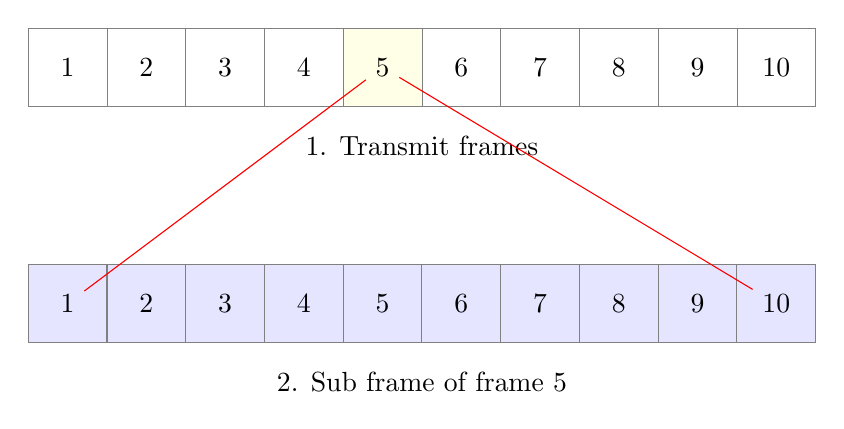
\begin{tikzpicture}
\begin{scope}
	\fill[yellow!10!white] (2, -2) rectangle (3, -1);
	\draw[step=1cm,gray,very thin] (-2,-2) grid (8,-1);
	\node at (-1.5, -1.5) {1};
	\node at (-0.5, -1.5) {2};
	\node at (0.5, -1.5) {3};
	\node at (1.5, -1.5) {4};
	\node (5) at (2.5, -1.5) {5};
	\node at (3.5, -1.5) {6};
	\node at (4.5, -1.5) {7};
	\node at (5.5, -1.5) {8};
	\node at (6.5, -1.5) {9};
	\node at (7.5, -1.5) {10};
	\node at (3,-2.5) {1. Transmit frames};
	\fill[blue!10!white] (-2, -5) rectangle (8, -4);
	\draw[step=1cm, gray, thin] (-2, -5) grid (8, -4);
	\node (1) at (-1.5, -4.5) {1};
	\node at (-0.5, -4.5) {2};
	\node at (0.5, -4.5) {3};
	\node at (1.5, -4.5) {4};
	\node at (2.5, -4.5) {5};
	\node at (3.5, -4.5) {6};
	\node at (4.5, -4.5) {7};
	\node at (5.5, -4.5) {8};
	\node at (6.5, -4.5) {9};
	\node (10) at (7.5, -4.5) {10};
	\draw[red] (5) -> (1);
	\draw[red](5) -> (10);
	\node at (3, -5.5) {2. Sub frame of frame 5};
\end{scope}
\end{tikzpicture}
\caption{Transmit frames and its sub frames in LTE}
\label{lteframe}
\end{figure}

\begin{figure}
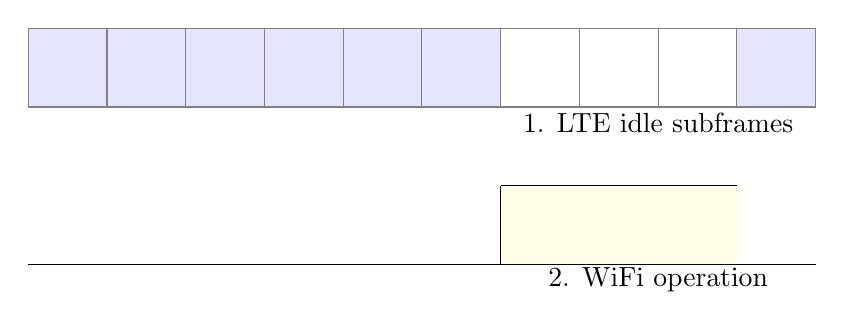
\begin{tikzpicture}
	\begin{scope}
	\fill[blue!10!white] (-2, -1) rectangle (4, 0);
	\fill[blue!10!white] (7,-1) rectangle (8, 0);
	\draw[step=1cm, gray, thin] (-2, -1) grid (8, 0);
	\node (10) at (7.5, -0.5) {};
	\node (11) at (6, -1.2) {1. LTE idle subframes};
	\draw (-2, -3) -- (8, -3);
	\draw(4, -3) grid (7, -2);
	\fill[yellow!10!white] (4, -3) rectangle (7, -2);
	\node (12) at (6, -3.2) {2. {WiFi} operation};
	\end{scope}
\end{tikzpicture}
\caption{{LTE-U}, {WiFi} coexistence using idle subframes in {LTE-U}}
\label{lteWiFicoex}
\end{figure}
A frame in {LTE-U} is divided into 10 subframes. Each subframe has 2 slots in it. Idle or blank subframe is transmitted with reduced power and is used only for control signalling. No user data will be available in this subframe. Figure \ref{lteframe} depicts the frames in LTE.
Figure \ref{lteWiFicoex} shows the coexistence mode of {WiFi} and {LTE-U} using idle subframes.
Initially {LTE-U} AP listens to the channel to determine the idle probability and collision probability among {WiFi} nodes.
\begin{equation}
					p_c^{AP} = \frac{N_c}{N_s}
\end{equation}
\begin{equation}
					p_i = \frac{N_i}{N_s}
\end{equation}
where N\textsubscript{c} is the number of collisions among {WiFi} nodes, N\textsubscript{i} is the number of idle periods, N\textsubscript{s} is the total number of slots listened. Number of {WiFi} nodes is estimated using the following equation. 
\begin{equation}				
					log_{(1-T_{NO})}p_i = \frac{(T_{NO} -1)(p_c^AP + p_i -1)}{p_iT_{NO}}
\end{equation}

where T\textsubscript{NO} is the transmission probability of {WiFi} node when {LTE-U} node does not transmit. Total system throughput(S\textsubscript{N\textsubscript{i}}) and Jain's fairness index(F\textsubscript{N\textsubscript{i}}) is defined by a reward function below. 
\begin{equation}
					R_{N_i} = \alpha S_{N_i} + (1 - \alpha)F_{N_i}
\end{equation}
$\alpha$ is the weighted factor.
F-LBT selects N\textsubscript{i} so that R\textsubscript{N\textsubscript{i}} is highest regardless of $\alpha$. Higher the number of idle subframes, lower the reward value since channel is not utilized effectively by the randomness in {WiFi} operation.

\subsubsection{{WiFi} and {WSN} coexistence model}
A {WiFi} node idle time is given by following equation.
\begin{equation}
					t_{idle} = DIFS + mT_{bs}
\end{equation}
where DIFS is the distributed co-ordinate function value that varies according to {WiFi} specification, m is random variable uniformly distributed in [0, 2\textsuperscript{CW}] with {CW} being the contention window. T\textsubscript{bs} is the backoff slot defined in specification.
If the channel is idle for t\textsubscript{idle}, {WiFi} node begins transmission followed by {SIFS} and {ACK}.

{WSN} node senses the channel for CCA period and transmits only if the channel is idle during CCA period. 
Transmit period of {WSN} nodes is given by
\begin{equation}
					{CCA} + t_p + SIFS + ACK
\end{equation}
However, if channel is busy, {WSN} node backs off incrementing the contention window by 1(backoff time is doubled) and retries after backoff until maximum contention window. Packet is then dropped if channel is still busy.

\cite{4436237} analyses the {MAC} operation of {WiFi} and {WSN} nodes in terms of power and timing aspects. {WiFi}, operating in {2.4Ghz} has higher power of transmit compared to {WSN}. This difference powers lead to three different ranges of in terms of power aspect.
\begin{itemize}
\item Both {WiFi} and {WSN} nodes can sense the power of each other on the channel.
	For {WSN} nodes to transmit, channel sensing time of {WSN} nodes should be less than {WiFi} channel sensing time as depicted in figure \ref{wsn1}.
\begin{figure}
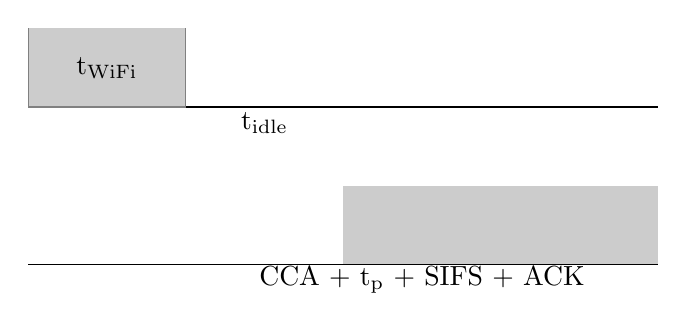
\begin{tikzpicture}
\begin{scope}
\draw (0, 0) -- (8,0);
\fill[gray!40!white] (0,0) rectangle (2, 1);
\draw[step=2cm, gray, thin] (0, 0) grid (2, 1);
\node at (1, 0.5) {t\textsubscript{WiFi}};
\node at (3, -0.2) {t\textsubscript{idle}};

\draw (0, -2) -- (8, -2);
\fill[gray!40!white] (4, -2) rectangle (8, -1);
\node at (5, -2.2) {CCA + t\textsubscript{p} + SIFS + ACK};
\end{scope}
\end{tikzpicture}
\caption{WSN transmission in case 1}
\label{wsn1}
\end{figure}
\begin{equation}
					CCA \leq DIFS + mT_{bs}
\end{equation}
For m $\geq$ 4 in 802.11b and m $\geq$ 12 in 802.11g, {WSN} node can transmit successfully.

\item {WSN} nodes can sense {WiFi} power while {WiFi} nodes cannot sense {WSN} nodes as shown in figure \ref{wsn2}
If {WSN} nodes transmit during idle period of {WiFi} nodes, transmission will be successful.
\begin{figure}
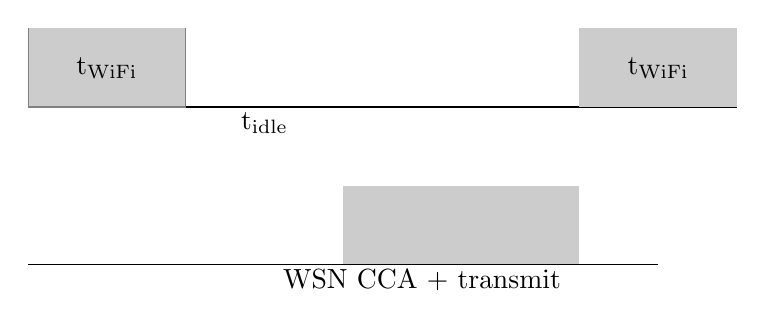
\begin{tikzpicture}
\begin{scope}
\draw (0, 0) -- (9,0);
\fill[gray!40!white] (0,0) rectangle (2, 1);
\draw[step=2cm, gray, thin] (0, 0) grid (2, 1);
\node at (1, 0.5) {t\textsubscript{WiFi}};
\node at (3, -0.2) {t\textsubscript{idle}};

\fill[gray!40!white] (7,0) rectangle (9, 1);
\node at (8,  0.5) {t\textsubscript{WiFi}};
\draw (0, -2) -- (8, -2);
\fill[gray!40!white] (4, -2) rectangle (7, -1);
\node at (5, -2.2) {WSN CCA + transmit};
\end{scope}
\end{tikzpicture}
\caption{WSN transmission in case 2}
\label{wsn2}
\end{figure}
\begin{equation}
					CCA + t_p + SIFS + ACK \leq DIFS + mT_{bs}
\end{equation}
This inequality doesn't hold. Transmission will be successful only when power at reception is high enough to recognize the transmission.

\item Both {WiFi} and  {WSN} nodes do not sense each other, however since {WiFi} has longer range, interferes with {WSN} transmission(blind transmissions).
In case of transmissions along with receipt of ACK, this case never holds for {WSN} nodes unless power at the reception is high enough to detect the transmission.

\end{itemize}

Throughput(S) of {WSN} node in presence of {WiFi} interference is given by the renewal process.
\begin{equation}
					S =  \frac{E[W_n]}{E[X]}
\end{equation}
\begin{equation}
					E[W_n] = pE[t_p]\sum_{i=0}^{4}{(1-p)}^i
\end{equation}
\begin{equation}
					E[X] = \sum_{i=0}^4[p{(1-p)}^i(\sum_{j=0}^iE[B_i] + (i + 1)CCA + E[t_p])] + (1-p)^5(\sum_{i=0}^4E[B_i] + 5CCA)
\end{equation}
\begin{equation}
					p = \frac{1}{CW_{min} + 1} \sum_{m=a}^{CW_{min}} \frac{DIFS + mT_{bs} - CCA}{E[t_w] + DIFS + mT_{bs}}
\end{equation}
where p is the probability of channel being idle for {WSN} transmission t\textsubscript{p}, t\textsubscript{w} is the transmission time of {WiFi} with SIFS and ACK. E[B\textsubscript{i}] is the expected value of backoff time B\textsubscript{i}(uniformly distributed in [0, 2\textsuperscript{BE\textsubscript{i}}]. a is either 4 or 12.

\subsubsection{Need for better coexistence model}
{F-LBT} based model uses {WiFi} collision probability to identify number of {WiFi} nodes in the network. Number of nodes is in turn used to estimate maximum reward. The key assumption here is, collisions as observed by {LTE AP} are due to {WiFi} transmissions only. Adding {WSN} into this model invalidates this assumption since collisions between {WiFi} and {WSN} need to be taken into account. 

Coexistence model for {WiFi} and {WSN} estimates the channel idle probability during {WSN} CCA so that {WSN} node can transmit. Since {WiFi} and {WSN} are {CSMA} based {MAC} protocols, certain level of fairness is built in. Key assumption here is channel is idle when {WSN} and {WiFi} nodes do not transmit. Introducing {LTE-U} into this model invalidates this assumption. {LTE-U} takes unfair advantage in accessing the channel thereby reducing the channel idle probability to almost zero.

\section{Proposed coexistence model}
Let us assume a {WSN} node needs to transmit 1 byte payload. {CCA} is 0.128ms, {SIFS} is 0.192ms, and at 250Kbps 1 byte payload transmit time is 0.448ms, ACK with 0 byte payload is 0.435ms.
Total air time in the best case(with random backoff set to 0) would be 
\begin{equation}
{CCA + 1 byte transmit time + SIFS + ACK transmit time} = 1.203ms
\end{equation}
In presence of {WSN}, minimum number of idle slots that {WSN} node requires would be atleast 2 to accommodate best case transmission.
{WSN} nodes' default retry limit is 4. Increasing the limit has more chances of finding the channel idle.
\begin{equation}
					N_{i} \geq 2 \label{rule 1}
\end{equation}

Consider the case where {WiFi} node needs to transmit 1500 byte payload. At 11Mbps rate, total time required to transmit and receive ack is around 1.374ms. At 6Mbps rate, total time is around 2.156ms. At 1Mbps rate, which is the lowest for {802.11 a/b/g/n}, total time is approximately 12.780ms. With {LTE-U}, medium is never idle more than idle slots in a 10ms frame.
So, {WiFi} operation needs to be adjusted to minimum rate of at least 6Mbps, and number of slots that should be left idle in 10ms {LTE-U} frame should be greater than 3.
\begin{equation}
					N_{i} \geq 3 \label{rule 2}
\end{equation}
{LTE-U} with {F-LBT} is capable of listening to the channel for a finite period of time. We leverage this to determine the transmit time of other protocols in the network i.e find the amount of time {T\textsubscript{p}} that {WiFi} and {WSN} nodes keep the medium busy. Let the total period of time be {T\textsubscript{total}}. $\frac{T\textsubscript{p}}{T\textsubscript{total}}$ gives the approximate transmit probability of {WiFi} and {WSN} nodes. Number of idle slots that {LTE-U} needs to set is directly proportional to this ratio.
\begin{equation}
					N_{i} \propto \frac{T\textsubscript{p}}{T\textsubscript{total}}
\end{equation}
N\textsubscript{i} could be identified as a simple linear function of $\frac{T\textsubscript{p}}{T\textsubscript{total}}$ with a range of [3, 10].
\begin{equation}
					N_{i} = K + \ceil{\alpha(\frac{T\textsubscript{p}}{T\textsubscript{total}})}
\end{equation}
where {K} is a constant and is set to 3 for the model described here, $\alpha$ is a fairness indicator for the network and ranges between 0 and 7.

\section{Analysis}
Probability of collision, which was the existing solution for coexistence with {LTE-U}, does not give enough insight on protocol accessing the shared medium. Probability of a protocol accessing the medium to transmit is given by probability of transmission. Current solution uses probability of transmission rather than probability of collision to determine the number of idle slots in {LTE-U} frame. Once idle slots are determined, {LTE-U} transmits in the non idle slots only. {WiFi} and {WSN} can safely coexist in the idle slots provided \ref{rule 1} and \ref{rule 2} are satisfied.
\subsection{Effect of $\alpha$}
$\alpha$ determines the weightage given to the fraction of the time other networks transmit. Higher the $\alpha$, higher the number of idle slots and higher the fairness given to other networks by {LTE-U}.
{WiFi} and {WSN} nodes share the medium without any idle perioids i.e. {T\textsubscript{p}} is equal to {T\textsubscript{total}}, depending on $\alpha$, N\textsubscript{i} could be set in the range from 3 to 9. If $\alpha$ is biased to {LTE-U}, N\textsubscript{i} is set to less than 5 and if $\alpha$ is biased towards the rest of the networks, N\textsubscript{i} is set to greater than 8.
{WiFi} and {WSN} nodes donot have any data to transmit i.e.  {T\textsubscript{p}} is 0. N\textsubscript{i} is set to 3 to accommodate minimum fairness in the network in case {WiFi} and {WSN} nodes wish to transmit. 
\subsection{Effect of higher retry limit in {WSN}}
Retry limit of {WSN} is set to higher value which increases the probability of {WSN} nodes transmission. However, this could cause reduction in lifetime of  battery operated devices. 
\subsection{Effect of lower limit on data rates of {WiFi}}
Minimum data rate of {WiFi} nodes is set to 6Mbps. Legacy devices which do not support high rates have very less chances of transmitting data. 

\section{Conclusion}
In this paper we have identified the shortcomings of two existing coexistence models and analysed why we need a new coexistence model for {LTE-U}, {WiFi} and {WSN} to coexist.
We have proposed a modification to {F-LBT} based {LTE-U} algorithm to determine the number of idle slots based on the channel occupancy time rather than probability of collision. This algorithm can be used in any model which adds any other protocols along with {WiFi} and {WSN}. \par

We have shown mathematically, increasing minimum data rate in {WiFi} and increasing retry limits of {WSN} yield better probability of transmissions in {WiFi+WSN} networks that coexist with {LTE-U}. In conclusion we have proposed a better coexistence model for {LTE-U}, {WiFi} and {WSN}. Future work includes experimental verifications and results of this proposal.
	\nocite{*}	
\bibliography{references}
\bibliographystyle{IEEEtran}

\end{document}
